\documentclass[a4paper,11pt,exos]{nsi} % COMPILE WITH DRAFT
\usepackage{pifont}
%\pagestyle{empty}

\begin{document}
\classe{\premiere spé}
\titre{Corrigé - Inéquations (1)}
\maketitle

Résoudre dans $\R$ les inéquations suivantes :
\begin{multicols}{2}
    \begin{enumerate}[itemsep=1em]
        \item $2x^2+4x+4< 0$
	    \item $-x^2+6x-14< 0$
	    \item $3x^2-3x-36< 0$
	    \item $-2x^2-14x-20\leqslant 0$
	    \item $-2x^2+12x-16>0$
	    \item $-x^2-4x-3\leqslant 0$
    \end{enumerate}
\end{multicols}

    %\begin{multicols}{2}

        \begin{enumerate}[itemsep=1em]
        \item Soit $P$ le polynôme défini pour tout $x$ de $\mathbb R$ par $P(x)=2x^2+4x+4$.\\On cherche à résoudre $P(x)< 0$.\\Pour cela, on cherche ses racines éventuelles.\\$\Delta = 4^2-4\times2\times4=-16$\\$\Delta<0$ donc le polynôme $P$ n'admet pas de racine.\\ Il est toujours du signe de $a=2>0$, donc $P(x)>0$ pour tout $x$ de $\mathbb{R}$.\\ On en déduit $S=\emptyset$.
        
        \item Soit $P$ le polynôme défini pour tout $x$ de $\mathbb R$ par $P(x)=-x^2+6x-14$.\\On cherche à résoudre $P(x)> 0$.\\Pour cela, on cherche ses racines éventuelles.\\$\Delta = 6^2-4\times(-1)\times(-14)=-20$\\$\Delta<0$ donc le polynôme $P$ n'admet pas de racine.\\ Il est toujours du signe de $a=-1<0$, donc $P(x)<0$ pour tout $x$ de $\mathbb{R}$.\\ On en déduit $S=\R$.
        
        \item Soit $P$ le polynôme défini pour tout $x$ de $\mathbb R$ par $P(x)=3x^2-3x-36$.\\On cherche à résoudre $P(x)< 0$.\\Pour cela, on cherche ses racines éventuelles.\\$\Delta = (-3)^2-4\times3\times(-36)=441$\\$\Delta>0$ donc le polynôme admet deux racines : $x_1 = \dfrac{-b-\sqrt{\Delta}}{2a}$ et $x_2 = \dfrac{-b+\sqrt{\Delta}}{2a}$.\\$x_1 =\dfrac{3-\sqrt{441}}{6}=-3$\\$x_2 =\dfrac{3+\sqrt{441}}{6}=4$\\On sait qu'un polynôme du second degré est du signe de $a$ à l'extérieur de ses racines.\\Comme $a=3>0 :$\\On peut résumer le signe du polynôme dans un tableau de signes :\\
        \begin{tikzpicture}[baseline, scale=0.5]
            \tkzTabInit[lgt=8,deltacl=0.8,espcl=5]{ $x$ / 2, $3x^2-3x-36$ / 2}{ $-\infty$, -3, 4, $+\infty$}
            \tkzTabLine{  , +, z, -, z, +}
            \end{tikzpicture}
        \\[.5em]
        Finalement $S=]-3;4[$.
        \item Soit $P$ le polynôme défini pour tout $x$ de $\mathbb R$ par $P(x)=-2x^2-14x-20$.\\On cherche à résoudre $P(x)\leq 0$.\\Pour cela, on cherche ses racines éventuelles.\\$\Delta = (-14)^2-4\times(-2)\times(-20)=36$\\$\Delta>0$ donc  le polynôme admet deux racines : $x_1 = \dfrac{-b-\sqrt{\Delta}}{2a}$ et $x_2 = \dfrac{-b+\sqrt{\Delta}}{2a}$.\\$x_1 =\dfrac{14-\sqrt{36}}{-4}=-5$\\$x_2 =\dfrac{14+\sqrt{36}}{-4}=-2$\\On sait qu'un polynôme du second degré est du signe de $a$ à l'extérieur de ses racines.\\Comme $a=-2<0 :$\\On peut résumer le signe du polynôme dans un tableau de signes :\\
        \begin{tikzpicture}[baseline, scale=0.5]
            \tkzTabInit[lgt=8,deltacl=0.8,espcl=5]{ $x$ / 2, $-2x^2-14x-20$ / 2}{ $-\infty$, -5, -2, $+\infty$}
            \tkzTabLine{  , -, z, +, z, -}
            \end{tikzpicture}
        \\[.5em]
        Finalement $S=]-\infty;-5]\cup[-2;+\infty[$.
        \item Soit $P$ le polynôme défini pour tout $x$ de $\mathbb R$ par $P(x)=-2x^2+12x-16$.\\On cherche à résoudre $P(x)>0$.\\Pour cela, on cherche ses racines éventuelles.\\$\Delta = 12^2-4\times(-2)\times(-16)=16$\\$\Delta>0$ donc le polynôme admet deux racines : $x_1 = \dfrac{-b-\sqrt{\Delta}}{2a}$ et $x_2 = \dfrac{-b+\sqrt{\Delta}}{2a}$.\\$x_1 =\dfrac{-12-\sqrt{16}}{-4}=2$\\$x_2 =\dfrac{-12+\sqrt{16}}{-4}=4$\\On sait qu'un polynôme du second degré est du signe de $a$ à l'extérieur de ses racines.\\Comme $a=-2<0$\\on en déduit le signe du polynôme dans un tableau de signes :\\
        \begin{tikzpicture}[baseline, scale=0.5]
            \tkzTabInit[lgt=8,deltacl=0.8,espcl=5]{ $x$ / 2, $-2x^2+12x-16$ / 2}{ $-\infty$, 2, 4, $+\infty$}
            \tkzTabLine{  , -, z, +, z, -}
            \end{tikzpicture}
        \\[.5em]
        Finalement $S=]2;4[$.
        \item Soit $P$ le polynôme défini pour tout $x$ de $\mathbb R$ par $P(x)=-x^2-4x-3$.\\On cherche à résoudre $P(x)\leq 0$.\\Pour cela, on cherche ses racines éventuelles.\\$\Delta = (-4)^2-4\times(-1)\times(-3)=4$\\$\Delta>0$ donc  le polynôme admet deux racines : $x_1 = \dfrac{-b-\sqrt{\Delta}}{2a}$ et $x_2 = \dfrac{-b+\sqrt{\Delta}}{2a}$.\\$x_1 =\dfrac{4-\sqrt{4}}{-2}=-3$\\$x_2 =\dfrac{4+\sqrt{4}}{-2}=-1$\\On sait qu'un polynôme du second degré est du signe de $a$ à l'extérieur de ses racines.\\Comme $a=-1<0 :$\\On peut résumer le signe du polynôme dans un tableau de signes :\\
        \begin{tikzpicture}[baseline, scale=0.5]
            \tkzTabInit[lgt=8,deltacl=0.8,espcl=5]{ $x$ / 2, $-x^2-4x-3$ / 2}{ $-\infty$, -3, -1, $+\infty$}
            \tkzTabLine{  , -, z, +, z, -}
            \end{tikzpicture}
        \\[.5em]
        Finalement $S=]-\infty;-3]\cup[-1;+\infty[$.
        \end{enumerate}
        %\end{multicols}
\end{document}